\subsection{CPU}\label{subsec:CPU}
Der eingesetzte Nios Prozessor ist für die Bedienung des Theremin und die Steuerung der Signalverarbeitungshardware zuständig. Die diversen eingesetzten IP Cores sind in den unten stehenden Kapiteln beschrieben.

\paragraph{JTAG, Timer und System ID}\mbox{}\\
Der JTAG IP Core ermöglicht das flüchtige Programmieren des Nios wie auch das Kommunizieren mit selbem für Debugging Zwecke. 
Durch den Einsatz des Timer IP Cores erhält der Nios einen Interval Timer um beispielsweise periodisch Interrupts zu generieren. 
In dem System ID IP Core ist die Systemidentifikationsnummer gespeichert. Diese wird benötigt um beim laden der Software sicherzustellen, dass das passende Hardware Image vorhanden ist.
Alle drei Komponenten sind mit Standardeinstellungen in das Nios System eingefügt worden.

\paragraph{Speicher}\mbox{}\\

Der Arbeitsspeicher ist ein externer 64MB SDRAM Chip IS42S16320D von ISSI. Für die Kommunikation mit dem Nios Prozessor ist der SDRAM Controller IP Core zuständig. Der Nios Prozessor kann über das Memory Mapped Interface mit dem Core Kommunizieren und so auf das SDRAM zugreifen. Da dieser Chip auf dem Entwicklungsboard sowieso vorhanden ist, haben wir uns gegen Onchip Speicher entschieden um Ressourcen zu sparen.\\

Das Hardware Image und der Programmcode ist auf dem Board enthaltenen Flash Speicher gespeichert. Dabei wird anders als bei dem nicht flüchtigen Programmieren nicht das SRAM Object File (.sof) geladen sondern ein JTAG Indirect Configuration File (.jic). Dieses kann in Quartus aus dem SRAM Object File und dem in Eclipse generierten HEX File erstellt werden. Anschliessend kann es über ein Serial Flash Loader Image über den USB Blaster auf den Flash geladen werden. Beim Einschalten des Gerätes wird zuerst das Hardwareimage ins FPGA geladen und anschliessend der Programmcode geholt. Auf Empfehlung von Dokumentationen von Intel haben wir uns dafür entschieden den Programmcode durch einen Bootcopier ins SDRAM zu kopieren. Abbildung \ref{img:FlashLayout} zeigt das Layout des Flash Speichers nach dem Programmieren. \cite{non_volatile}

\begin{figure}[h!]
	\centering
	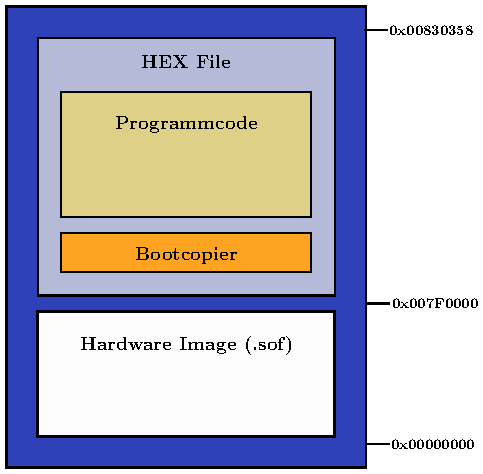
\includegraphics[width=0.45\textwidth]{FlashLayout.pdf}
	\caption{Layout des Flash Speichers} 
	\label{img:FlashLayout}
\end{figure}  

\paragraph{LCD Controller \& Reset}\mbox{}\\

Für das beschreiben des LCD ist die von terasIC bereitgestellte VHDL Komponente LT24\_Controller zuständig. Dieser kann über das Memory Mapped Interface von dem Nios Prozessor gesteuert werden. Das verwendete Display LT24 von terasIC enthält für das Schreiben des LCD den LCD Treiber ILI9341 von ILITEK. Dieser Chip wird durch den LT24\_Controller über das parallele \SI{16}{Bit} Interface gesteuert. Weiter kann der LCD Chip über den PIO Core LCD Reset zurückgesetzt werden. Wie diese beiden Komponenten in Software angesteuert werden ist in Kapitel \ref{subsec:Drivers} genauer beschrieben. \cite{LCD_Chip}

\paragraph{Touchscreen}\mbox{}\\
Der Touch Screen Digitizer AD7843 von Analog Devices misst den resistiven Touchscreen des LCD aus und übermittelt die digitalisierten Koordinaten über SPI an den Prozessor. Der Nios Kommuniziert dabei über drei verschiedene IP Cores mit diesem Chip. Der SPI Core \textit{Touch SPI} für die Datenübertragung, der PIO Core \textit{Touch Busy} um den Beschäftigungsstatus des Chips zu wissen und den zweiten PIO Core \textit{Touch Interrupt}, welcher den Nios über eine Betätigung des Touchscreens informert. Bei einer Berührung des Touchscreens löst \textit{Touch Interrupt} beim Nios Prozessor einen Interrupt aus, welcher sofort die Koordinaten über SPI anfordert. \cite{Touch_ADC}